\documentclass[12pt,a4paper]{article}

\usepackage{hyperref}
\usepackage{listings}
\usepackage{graphicx}
\usepackage{cleveref}
\usepackage{xcolor} % For colors
\usepackage[textheight=8in]{geometry}

% Define colors for syntax highlighting
\definecolor{keywordcolor}{rgb}{0.5, 0.0, 0.5}
\definecolor{stringcolor}{rgb}{0.2, 0.6, 0.2}
\definecolor{commentcolor}{rgb}{0.5, 0.5, 0.5}

\title{SPM - Assignment 1}
\author{Angelo Savino}

\begin{document}

\maketitle

\section{Handouts}
This assignment consisted in writing an optimized version of the softmax function. The three versions we compared are the following:
\begin{itemize}
    \item \texttt{softmax\_plain}: Basic version of the softmax function that does not employ any kind of SIMD optimization.
    \item \texttt{softmax\_auto}: Version of the softmax function that relies on compiler optimizations to produce AVX code. 
    \item \texttt{softmax\_avx}: Hand-optimized version of the code that uses AVX intrinsic.
\end{itemize}

\section{Softmax\_auto}
The \texttt{softmax\_auto} binary was compiled using the \texttt{-march=native} and \texttt{-ffast-math} compiler flags, to allow for the use of respectively AVX instructions and fast math code.
Also at the start of the \texttt{softmax\_auto()} function, the input and output vector have been tagged with \texttt{\_\_restricted\_\_}, to allow the compiler to make better assumptions about the code we will need to generate. 

\section{Softmax\_avx}
The hand-optimized version optimizes all loops using avx instructions. The first loop is the one present in the \texttt{find\_max} function, where we load 8 floats per iteration into a AVX2 register using \texttt{\_mm256\_loadu\_ps}, then we find the max for each slot using \texttt{\_mm256\_max\_ps}. Finally, we store the current max values we found in a temporary array of size 8, and we find the max value over the elements by iterating over them. 

In the same fashion, we load compute the exponentials in groups of 8 by first subtracting to each of them the max value using \texttt{\_mm256\_sub\_ps}, then compute the exponential using \texttt{exp256\_ps}. Once we do this, we save the values into the output vector, and we also sum them up into another register which will be reduced to the sum of all exponentials at the end.

At last, we divide each element by the computed sum of the exponentials using the \texttt{\_mm256\_div\_ps}.

\section{Performance Comparison}
The final performance comparison is summarized by \cref{fig:comparison}. As we can see, there is not much difference between the version when the size of the vector $K$ is sufficiently small. 

When vectors get bigger ($K > 10^3$), we can start noticing a difference in execution time. The unoptimized version is the slowest, while the auto optimized one results in a speedup of about 2.7x for the largest K we tested ($K = 10^{8}$) and the hand-optimized one improves our times by an additional 1.24x (3.3x faster than plain).

Overall, \texttt{softmax\_avx} is the best performing implementation, but it comes at the cost of portability, meaning that if we would like to run our code on other machines that are not provided of the AVX2 extension, we would be better off using our auto-optimized version if we can accept slightly higher run times.


\begin{figure}[h]
    \centering
    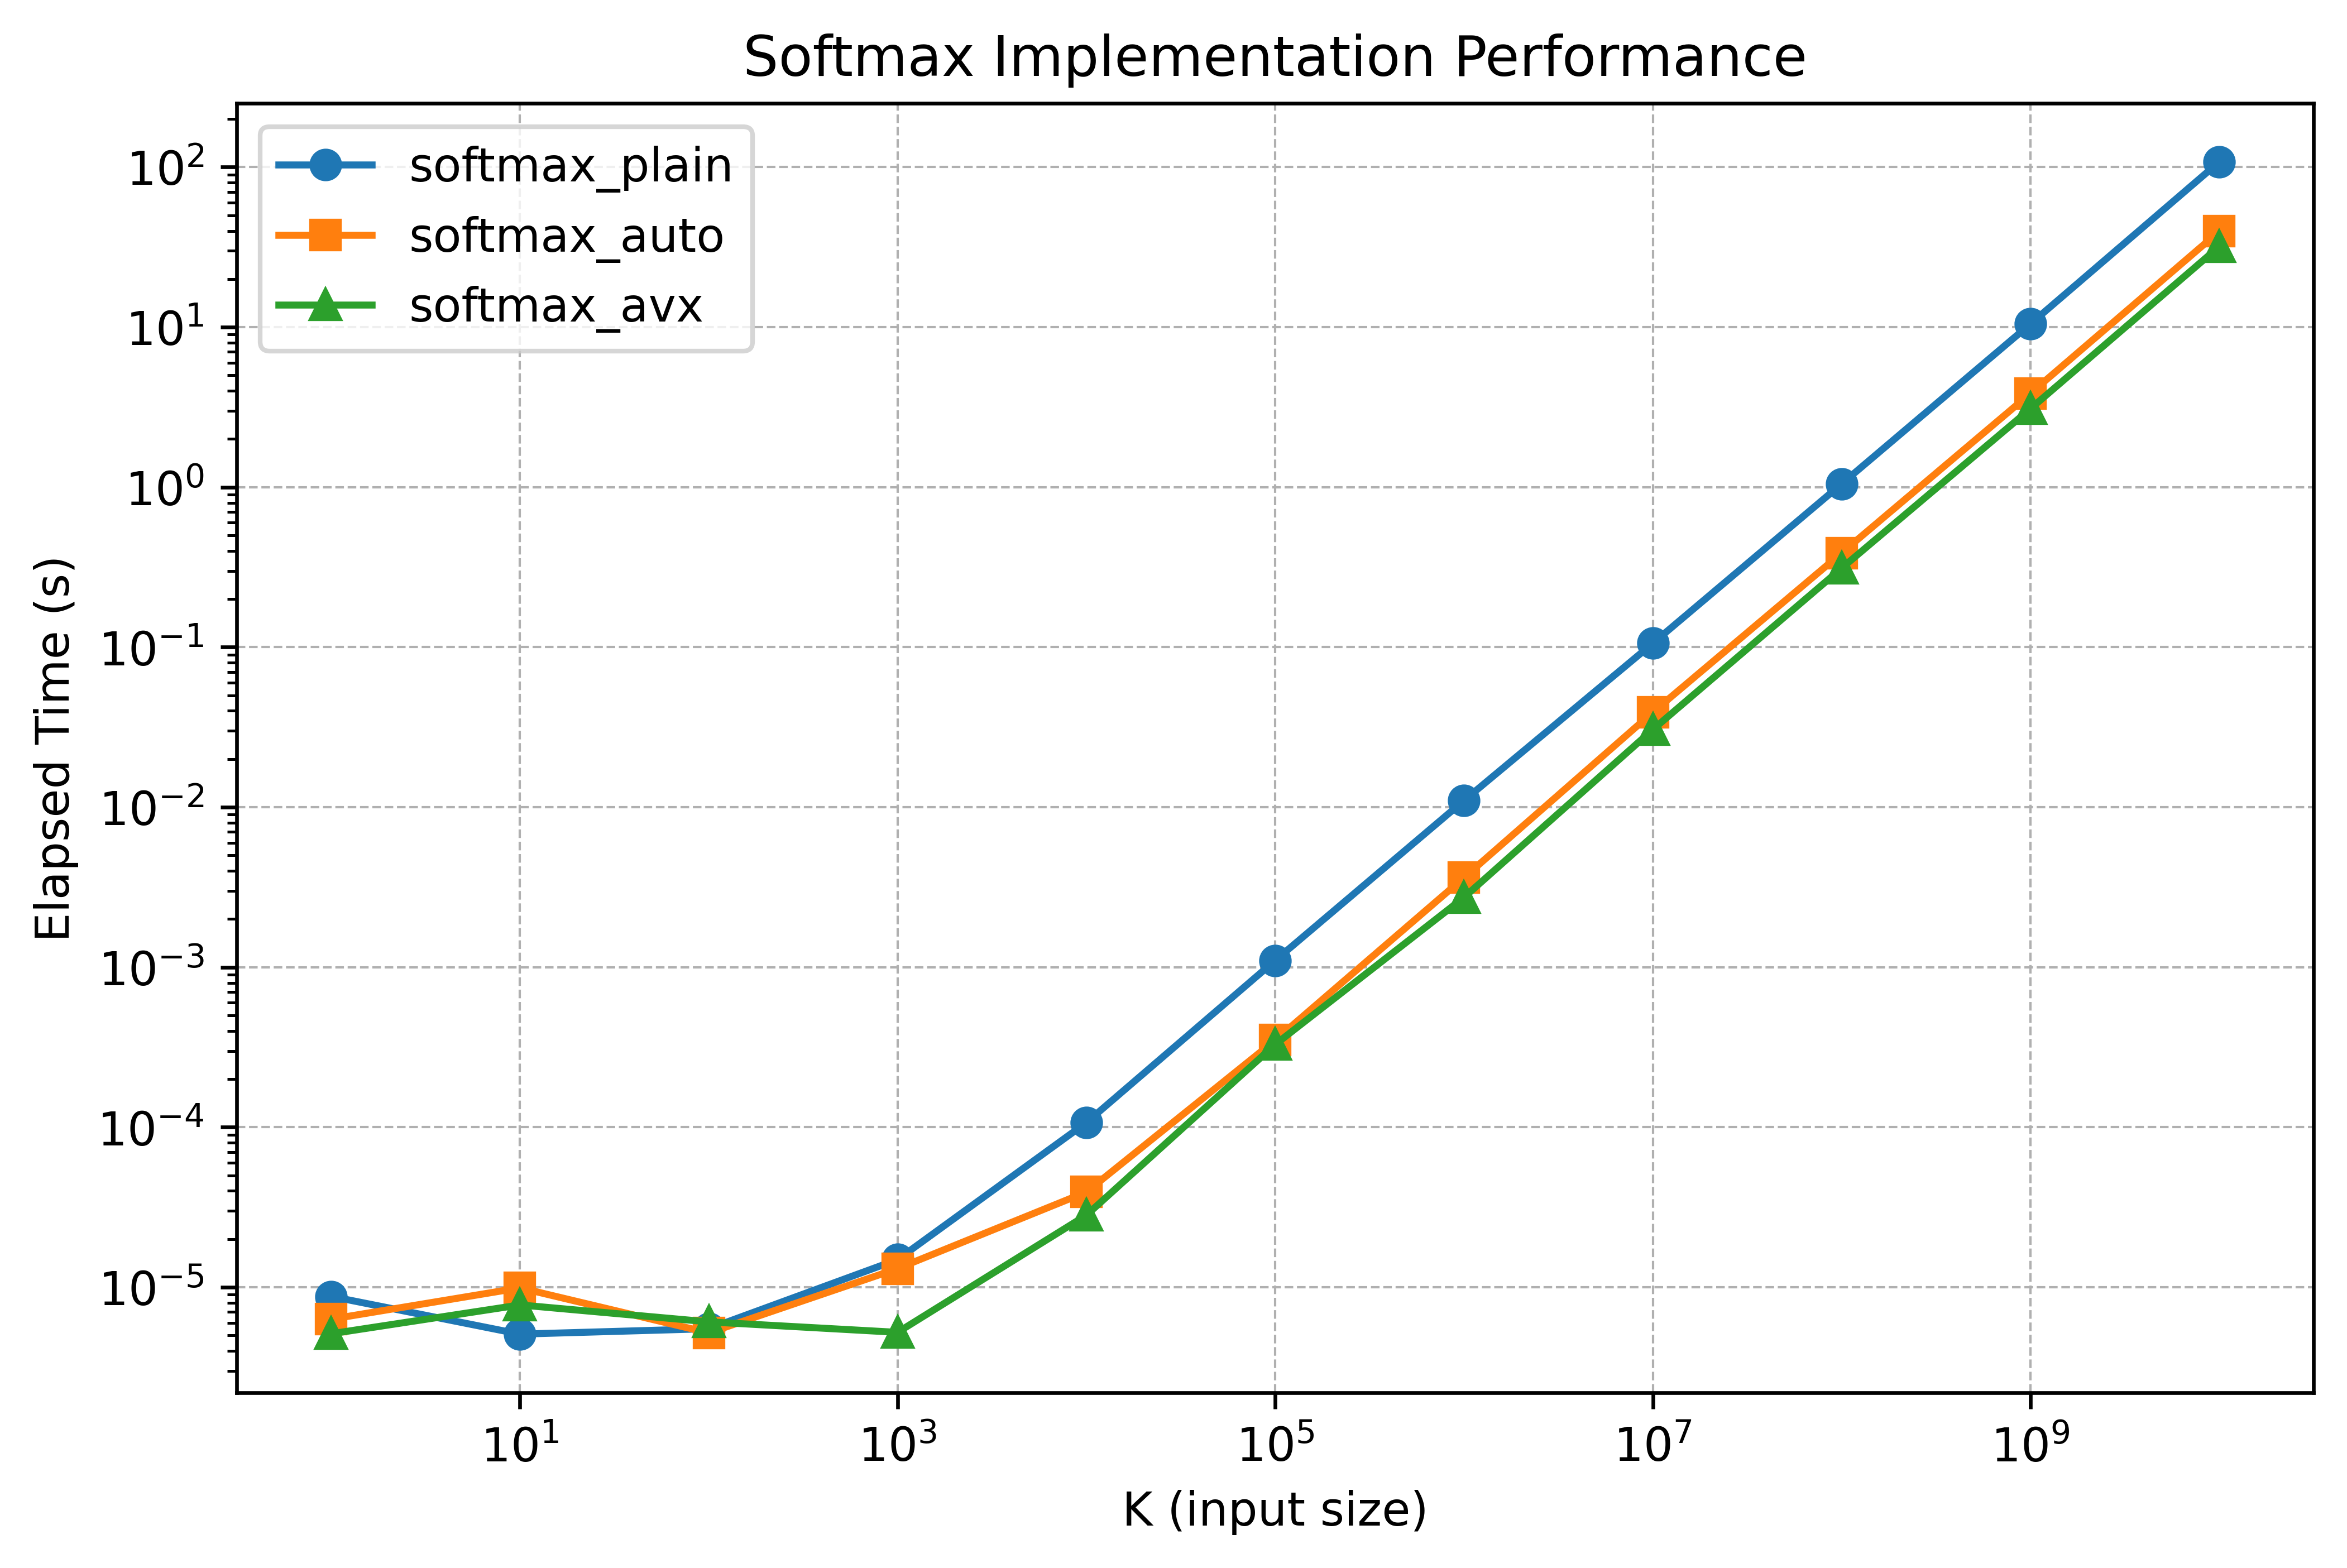
\includegraphics[width=0.75\textwidth]{notebooks/rep1_softmax_performance.png} 
    \caption{Comparison between all variants of softmax}   
    \label{fig:comparison}
\end{figure}

\end{document}